\documentclass[tikz,border=8pt]{standalone}
\usepackage{amsmath,amssymb}
\usetikzlibrary{arrows.meta,automata,positioning,quotes}
\begin{document}
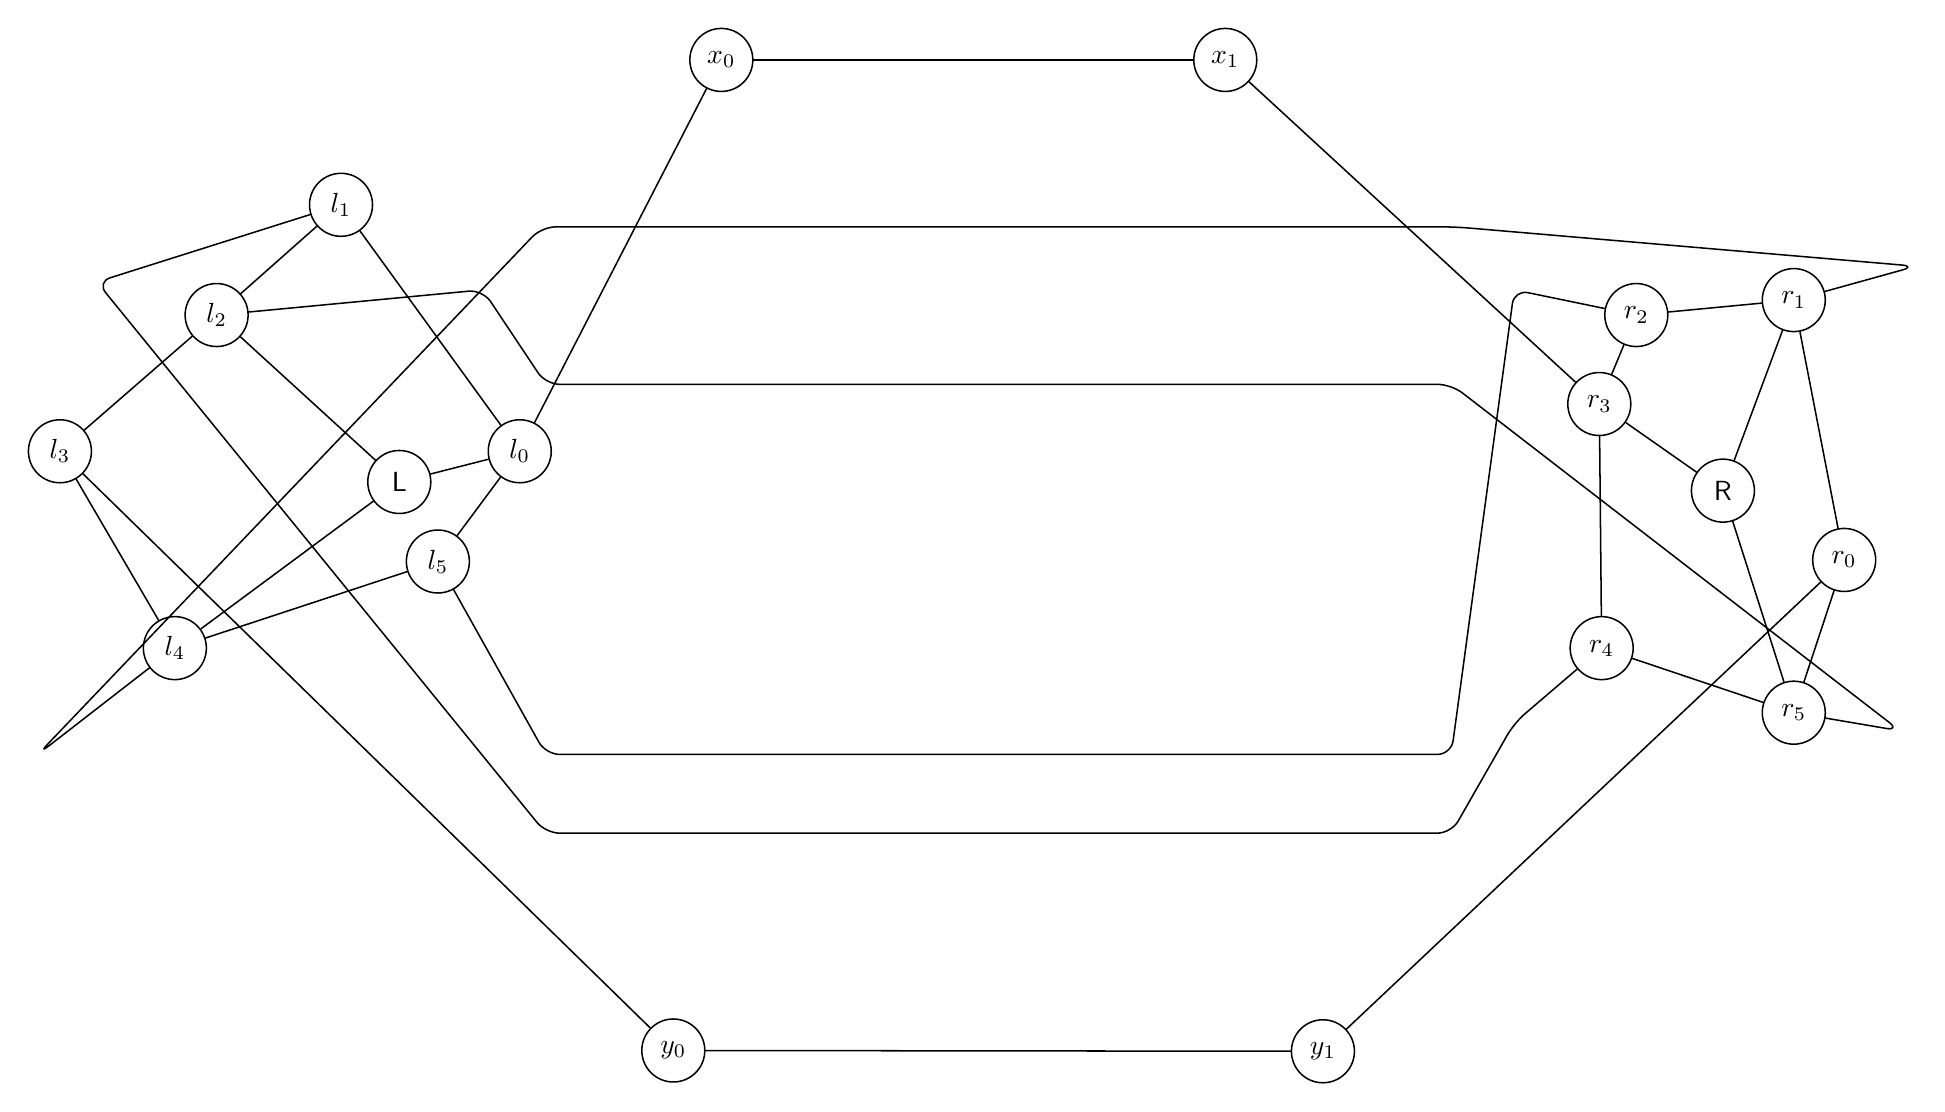
\begin{tikzpicture}[x=1cm,y=1cm]
\tikzset{
  graphnode/.style={circle,draw=black,line width=0.55pt,minimum size=8mm,inner sep=1pt,font=\sffamily},
  graphedge/.style={draw=black,line width=0.55pt,line cap=round,line join=round},
  directed/.style={graphedge,-{Stealth[length=2.4mm,width=2.0mm]}},
  undirected/.style={graphedge}
}
\node[graphnode] (n_L) at (-7.61,0.31) {L};
\node[graphnode] (n_l0) at (-6.08,0.70) {$l_{0}$};
\node[graphnode] (n_l1) at (-8.35,3.83) {$l_{1}$};
\node[graphnode] (n_l2) at (-9.93,2.43) {$l_{2}$};
\node[graphnode] (n_l3) at (-11.92,0.70) {$l_{3}$};
\node[graphnode] (n_l4) at (-10.46,-1.80) {$l_{4}$};
\node[graphnode] (n_l5) at (-7.12,-0.70) {$l_{5}$};
\node[graphnode] (n_R) at (9.20,0.20) {R};
\node[graphnode] (n_r0) at (10.74,-0.68) {$r_{0}$};
\node[graphnode] (n_r1) at (10.10,2.62) {$r_{1}$};
\node[graphnode] (n_r2) at (8.10,2.43) {$r_{2}$};
\node[graphnode] (n_r3) at (7.63,1.30) {$r_{3}$};
\node[graphnode] (n_r4) at (7.66,-1.80) {$r_{4}$};
\node[graphnode] (n_r5) at (10.10,-2.62) {$r_{5}$};
\node[graphnode] (n_x0) at (-3.52,5.67) {$x_{0}$};
\node[graphnode] (n_x1) at (2.88,5.67) {$x_{1}$};
\node[graphnode] (n_y0) at (-4.13,-6.91) {$y_{0}$};
\node[graphnode] (n_y1) at (4.12,-6.92) {$y_{1}$};
\draw[undirected] (n_l0) -- (n_l1);
\draw[undirected] (n_l1) -- (n_l2);
\draw[undirected] (n_l2) -- (n_l3);
\draw[undirected] (n_l3) -- (n_l4);
\draw[undirected] (n_l4) -- (n_l5);
\draw[undirected] (n_l5) -- (n_l0);
\draw[undirected] (n_L) -- (n_l0);
\draw[undirected] (n_L) -- (n_l2);
\draw[undirected] (n_L) -- (n_l4);
\draw[undirected] (n_r0) -- (n_r1);
\draw[undirected] (n_r1) -- (n_r2);
\draw[undirected] (n_r2) -- (n_r3);
\draw[undirected] (n_r3) -- (n_r4);
\draw[undirected] (n_r4) -- (n_r5);
\draw[undirected] (n_r5) -- (n_r0);
\draw[undirected] (n_R) -- (n_r1);
\draw[undirected] (n_R) -- (n_r3);
\draw[undirected] (n_R) -- (n_r5);
\draw[undirected] (n_l0) -- (n_x0);
\draw[undirected] (n_x0) -- (n_x1);
\draw[undirected] (n_x1) -- (n_r3);
\draw[undirected] (n_l3) -- (n_y0);
\draw[undirected] (n_y0) -- (n_y1);
\draw[undirected] (n_r0) -- (n_y1);
\draw[undirected,rounded corners=5pt] (n_l1) -- (-11.45,2.85) -- (-5.75,-4.15) -- (5.75,-4.15) -- (6.55,-2.75) -- (n_r4);
\draw[undirected,rounded corners=5pt] (n_l2) -- (-6.55,2.75) -- (-5.75,1.55) -- (5.75,1.55) -- (11.45,-2.85) -- (n_r5);
\draw[undirected,rounded corners=5pt] (n_l4) -- (-12.20,-3.15) -- (-5.80,3.55) -- (5.80,3.55) -- (11.65,3.05) -- (n_r1);
\draw[undirected,rounded corners=5pt] (n_l5) -- (-5.75,-3.15) -- (5.75,-3.15) -- (6.55,2.75) -- (n_r2);
\end{tikzpicture}
\end{document}
